\documentclass[../main.tex]{subfiles}
\begin{document}

\setcounter{footnote}{0} 

\chapter{Appendices}

\section{ML Representations}
\subsection{SOAP} \label{section::soap_derivation}

A SOAP vector\cite{Bartok2013} $\boldsymbol{p}$ is given by concatenating elements

\begin{equation}
	p_{nn'l}^{Z_1, Z_2} = \pi \sqrt{\frac{8}{2l + 1}} \sum_m \left(c_{nlm}^{Z_1}\right)^* c_{n'lm}^{Z_2}
\end{equation}

for every pair of atoms with atomic number $Z$ and the coefficients ($c_{nlm}$) are of radial and angular basis functions centred a particular atom given by

\begin{equation}
	c_{nlm}^Z = \int_\mathcal{R} g_n(r) Y_{lm}(\phi,\theta) \rho^Z(\boldsymbol{r})\; \text{d}V
\end{equation}
where the atomic density is given as a sum over 3D Gaussian centred on each atom $i$ 
\begin{equation}
	\rho^Z(\boldsymbol{r}) = \sum_{i \in \{Z\}} \exp\left(-\frac{|\boldsymbol{r} - \boldsymbol{R}_i|^2}{2\sigma_\text{at}^2}\right)
\end{equation}
A component of the neighbour density is then ($a := 1/2\sigma_\text{at}^2$) 
% https://journals.aps.org/prb/pdf/10.1103/PhysRevB.87.184115
% https://iopscience.iop.org/article/10.1088/0953-4075/22/1/004/pdf
\begin{equation}
	\text{e}^{-a|\boldsymbol{r} - \boldsymbol{R}_i|^2} = 4\pi \text{e}^{-a(r^2+R_i^2)}i_l(2arR_i) \sum_{l'm'}Y_{l'm'}(\phi, \theta) Y_{l'm'}^*(\boldsymbol{R}_i)
\end{equation}
inserting and using the orthogonality of the spherical harmonics integrated over theta and phi
\begin{equation}
	\begin{split}
		c_{nlm}^Z &= \int_\mathcal{R} g_n(r) Y_{lm}(\phi,\theta)  \sum_{i \in \{Z\}} \exp\left(-a|\boldsymbol{r} - \boldsymbol{R}_i|^2\right) \text{d}V \\
		&= \sum_{i \in \{Z\}} \int_\mathcal{R} g_n(r) Y_{lm}(\phi,\theta) \exp\left(-a|\boldsymbol{r} - \boldsymbol{R}_i|^2\right) \text{d}V \\
		&=  4\pi \sum_{i \in \{Z\}}\sum_{l'm'} \int_\mathcal{R} g_n(r) Y_{lm}(\phi,\theta) \text{e}^{-a(r^2+R_i^2)}i_l(2arR_i)Y_{l'm'}(\phi, \theta) Y_{l'm'}^*(\boldsymbol{R}_i)  \text{d}V \\
		&=4\pi \sum_{i \in \{Z\}}Y_{lm}^*(\boldsymbol{R}_i) \int_\mathcal{\tilde{R}} g_n(r) \text{e}^{-a(r^2+R_i^2)}i_l(2arR_i)r^2\; \text{d}r
	\end{split}
\end{equation}
where $i_l$ is a modified spherical Bessel function of the first kind. Inserting a orthonormal radial basis as $g_n(r)$
\begin{equation}
	\begin{split}
		c_{nlm}^Z &=4\pi \sum_{i \in \{Z\}}Y_{lm}^*(\boldsymbol{R}_i) \int_\mathcal{\tilde{R}} \sum_{n'}^{n_\text{max}} \beta_{nn'l}r^l e^{-\alpha_{n'l}r^2}\text{e}^{-a(r^2+R_i^2)} i_l(2arR_i)r^2\; \text{d}r \\
		&= 4\pi \sum_{i \in \{Z\}}Y_{lm}^*(\boldsymbol{R}_i)\text{e}^{-aR_i^2} \sum_{n'}^{n_\text{max}} \beta_{nn'l}\int_\mathcal{\tilde{R}} r^{l + 2}  \text{e}^{-(\alpha_{n'l} + a)r^2} i_l(2arR_i)\; \text{d}r
	\end{split}
\end{equation}

Evaluating the integral where $b  := \alpha_{n'l} + a$ and $c_i:= 2aR_i$

\begin{equation}
	I_{iln'} = \int_0^\infty r^{l+2} \text{e}^{-br^2}i_l(c_i r)\; \text{d}r
\end{equation}

using $i_\lambda(z) = i^{-\lambda}j_\lambda(iz)$ where from Gradshteyn and Ryzhik\cite{Gradshteyn2007} 
% https://arxiv.org/pdf/1908.07374.pdf

\[\int_0^\infty x^{\lambda + 2}\text{e}^{-k_1x^2}j_\lambda(k_2x) \text{d}x =  
\sqrt{\frac{\pi}{2}} \frac{k_2^\lambda}{(2k_1)^{\lambda + 3/2}}\exp\left(-\frac{k_2^2}{4k_1}\right)\]

so the required integral is with $\lambda = l, k_1 = b, k_2 = ic_i$

\begin{equation}
	\begin{split}
		I_{iln'} &= \sqrt{\frac{\pi}{2}} \frac{c_i^l}{(2b)^{l+3/2}}\exp\left(\frac{c_i^2}{4b}\right) \\
		&=  \sqrt{\frac{\pi}{2}} \frac{(2aR_i)^l}{(2(\alpha_{n'l} + a))^{l+3/2}}\exp\left(\frac{(aR_i)^2}{\alpha_{n'l} + a}\right)
	\end{split}
\end{equation}
so then

\begin{equation}
	\begin{split}
		c_{nlm}^Z &= \sqrt{8\pi^3} \sum_{i \in \{Z\}}Y_{lm}^*(\boldsymbol{R}_i)\,\text{e}^{-aR_i^2} \sum_{n'}^{n_\text{max}} \beta_{nn'l} \frac{(2aR_i)^l}{(2(\alpha_{n'l} + a))^{l+3/2}}\exp\left(\frac{(aR_i)^2}{\alpha_{n'l} + a}\right)
	\end{split}
\end{equation}

Using real spherical harmonic functions 

\begin{equation}
	Y_{l,m}(\theta, \phi) = \begin{cases}
		\sqrt{2}(-1)^m \,\text{Im}\{Y_l^{|m|}(\theta, \phi)\} &\quad \text{if } m < 0 \\
		1 &\quad \text{if } m = 0 \\
		\sqrt{2}(-1)^m\,\text{Re}\{Y_l^{m}(\theta, \phi)\} &\quad \text{if } m > 0 \\
	\end{cases}
\end{equation}
where
\begin{equation}
	Y_l^m (\theta, \phi) = \sqrt{\frac{(2l+1)(l- m)!}{4\pi (l+m)!}} P_l^{m}(\cos\theta)e^{im\phi}
\end{equation}




\section{Solution Phase Entropy}
\subsection{Partition Functions} \label{section::appendix_igm_partition_functions}

Approximating the sum with an integral, which is valid provided the gaps between energy levels is small, then
\begin{equation}
	q_\text{trans} \approx \int_0^\infty dn_x\;dn_y\;dn_z\; \exp{ {\Big \{} -{\beta}\cdot  \frac{\hbar^2 \pi^2}{2ml^2}(n_x^2 + n_y^2 + n_z^2)}{\Big \}}
\end{equation}

Converting into spherical polar coordinates with $n_x^2 + n_y^2 + n_z^2 = n_r^2$ and integrating over $n_\theta$ and $n_\phi$ in the positive octant
\begin{equation}
	q_\text{trans} \approx \frac{1}{8} \cdot 4\pi \int_0^\infty dn_r\; n_r^2\exp{ {\Big \{} -{\beta}\cdot  \frac{\hbar^2 \pi^2}{2ml^2}n_r^2}{\Big \}}
\end{equation}

Using the standard integral $\int_{0}^{\infty} dx\; x^2 e^{-ax^2} = \sqrt{\pi}/4a^{3/2}$ and noting $V = l^3$
\begin{equation}
	\begin{aligned}
		q_\text{trans} &\approx \frac{\pi}{2} \cdot \frac{\sqrt{\pi}}{4} {\Big (} \frac{\hbar^2 \pi^2\beta}{2ml^2} {\Big )}^{-3/2} \\
		&\approx \pi^{3/2} {\Big (} \frac{ml^2}{2\hbar^2 \pi^2\beta} {\Big )}^{3/2} \\
		&\approx {\Big (} \frac{2\pi m k_B T}{h^2} {\Big )}^{3/2} V 
		\label{q_trans_pib}
	\end{aligned}
\end{equation}

Interestingly, \eqref{q_trans_pib} is identical to that obtained classically \eqref{q_trans_pib_classical}.

\begin{equation}
	\begin{aligned}
		q_\text{trans, c} &= \frac{1}{h^{3}}\int\int e^{-\beta H(\boldsymbol{p}, \boldsymbol{x})} \; d\boldsymbol{p}^{3} d\boldsymbol{x}^{3} \\
		&= \frac{1}{h^{3}}\int_{-\infty}^\infty e^{-\beta \boldsymbol{p}^2/2m} \; d\boldsymbol{p}^{3} \int_0^l e^{-\beta \cdot 0} \;  d\boldsymbol{x}^{3} \\
		&= \frac{1}{h^{3}} {\Big \{}  \int_{-\infty}^\infty e^{-\beta {p_k}^2/2m} \; d{p_k} {\Big \}}^3 {\Big \{}  \int_0^l  \;  dx_k {\Big \}}^3 \\
		&= \frac{l^3}{h^{3}} {\Big \{}  \sqrt{\frac{\pi}{1/(2 k_b T)}} {\Big \}}^3 \\
		&={\Big (} \frac{2\pi m k_B T}{h^2} {\Big )}^{3/2} V 
		\label{q_trans_pib_classical}
	\end{aligned}
\end{equation}

\subsection{Classical Truncated Harmonic Oscillator}

The classical entropy of the truncated harmonic oscillator with potential energy 
\begin{equation}
	V(x) = \begin{cases}
		\frac{1}{2}m\omega^2x^2 &\text{if} \quad x > -r_e \\
		+\infty &\text{if} \quad x \le -r_e
	\end{cases} 
\end{equation}
is derived as follows. First the classical partition function is\footnote{Using $\int_{a}^{+\infty}  e^{-bx^2} dx = \sqrt{\pi/b}\;\text{erfc}(a\sqrt{b})/2$}

\begin{equation}
	\begin{aligned}
		Z_c &= \frac{1}{h}\int_{-\infty}^\infty \; dp\int_{-\infty}^{\infty} \; dx \; e^{-\beta E(x,p)} \\
		&= \frac{1}{h}\int_{-\infty}^\infty \; dp \; e^{-\beta p^2/2m} \int_{-\infty}^{\infty} \; dx \; e^{-\beta V(x)} \\
		&= \frac{1}{h}\int_{-r_e}^\infty \; dp \; e^{-\beta p^2/2m} \int_{-r_e}^{\infty} \; dx \; e^{-\beta m\omega^2x^2/2} \\
		&=\frac{1}{h}\cdot \frac{\sqrt{\pi}\;\text{erfc}(-r_e \sqrt{\beta/2m})}{2\sqrt{\beta/2m}}\cdot \frac{\sqrt{\pi}\;\text{erfc}(-r_e \sqrt{\beta m\omega^2/2})}{2\sqrt{\beta m\omega^2/2}} \\
		&=\frac{\pi k_b T}{2h\omega} \;\text{erfc}(-r_e \sqrt{\beta/2m})\;\text{erfc}(-r_e \sqrt{\beta m\omega^2/2})
	\end{aligned}
\end{equation}

where $\text{erfc}(x)$ is the complementary error function. The derivative with respect to temperature for $a = r_e^2/ 2k_B m$ and $b = r_e^2m\omega^2/2k_B$ is 

\begin{equation}
	\begin{aligned}
		\frac{d Z_c}{dT} &= \frac{d}{dT} {\Big \{} \frac{\pi k_b T}{2h\omega} \;\text{erfc}(- \sqrt{a/T})\;\text{erfc}(- \sqrt{b/T}) {\Big \}} \\
		&= \frac{ k_b}{4\hbar\omega} {\Bigg (} \text{erfc}(- \sqrt{a/T})\;\text{erfc}(- \sqrt{b/T}\,) - \frac{b e^{-b/T} \; \text{erfc}(-\sqrt{a/T})}{\sqrt{b\pi T}} - \frac{a e^{-a/T} \; \text{erfc}(-\sqrt{b/T})}{\sqrt{a\pi T}} {\Bigg )}
	\end{aligned}
\end{equation}

\subsection{Classical Morse Oscillator}

The classical entropy of a Morse oscillator as a model of a chemical bond requires an upper bound to the total energy to prevent the configurational integral becoming unbounded. For a total energy 
\begin{equation}
	E(p, x) = \frac{p^2}{2m} + D_e (1 - e^{-a(r-r_e)})^2
\end{equation}
where $r$ is the bond length and $r_e$ the equilibrium bond length. The maximum energy is the dissociation energy of the bond ($D_e$) such that the the momentum is bounded
\begin{equation}
	E(x, p) < D_e \qquad \implies \qquad p_\pm = \pm \sqrt{2mD_e(1 - (1-e^{-ax})^2)}
\end{equation}
where $x$ is the displacement from equilibrium, with $x > -\frac{1}{a}\ln(2)$ to ensure the momentum is real. 

The classical partition function is then\footnote{Using $\int_{-a}^{+a}  e^{-bx^2} dx = \sqrt{\pi/b}\;\text{erf}(a\sqrt{b})$ and that $\text{erf}$ is an even function.}

\begin{equation}
	\begin{aligned}
		Z_c &= \frac{1}{h}\int_{-\infty}^\infty \; dp\int_{-\infty}^{\infty} \; dx \; e^{-\beta E(x,p)} \\
		&= \frac{1}{h}\int_{p_-}^{p_+} \int_{-\infty}^{\infty}\; e^{-\beta \{{p^2}/{2m} + D_e (1 - e^{-ax})^2\}}  \; dx  \; dp \\
		&= \frac{1}{h}\int_{p_-}^{p_+} \int_{-\infty}^{\infty}\; e^{-\beta {p^2}/{2m}} e^{-\beta D_e (1 - e^{-ax})^2}  \; dx  \; dp \\
		&= \frac{1}{h} \int_{-\infty}^{\infty}\;\int_{p_-}^{p_+}\; e^{-\beta {p^2}/{2m}} e^{-\beta D_e (1 - e^{-ax})^2}  \; dx  \; dp \\
		&= \frac{1}{h} \int_{-\infty}^{\infty}\; e^{-\beta D_e (1 - e^{-ax})^2}  \cdot \frac{\sqrt{\pi}\;\text{erf}(p\sqrt{\beta/2m})}{\sqrt{\beta/2m}} \Bigg|_{p_-}^{p_+} \; dx \\
		&= \frac{2}{h}\sqrt{\frac{2m\pi}{\beta}} \int_{-\frac{1}{a}\ln(2)}^{\infty}\; e^{-\beta D_e (1 - e^{-ax})^2}   \;\text{erf}(p_+\sqrt{\beta/2m}) \; dx \\
		&= \frac{2}{h}\sqrt{\frac{2m\pi}{\beta}} \int_{-\frac{1}{a}\ln(2)}^{\infty}\; e^{-\beta D_e (1 - e^{-ax})^2}   \;\text{erf}{\Big (} \sqrt{\beta D_e(1 - (1-e^{-ax})^2)}{\Big )} \; dx 
	\end{aligned}
	\label{morse_pf_integral}
\end{equation}

Although \eqref{morse_pf_integral} has no analytical solution, the integrand is smooth allowing for efficient numerical evaluation (\figurename{ \ref{morse_pf_integrand_vs_x}}).

\begin{figure}[h!]
	\centering
	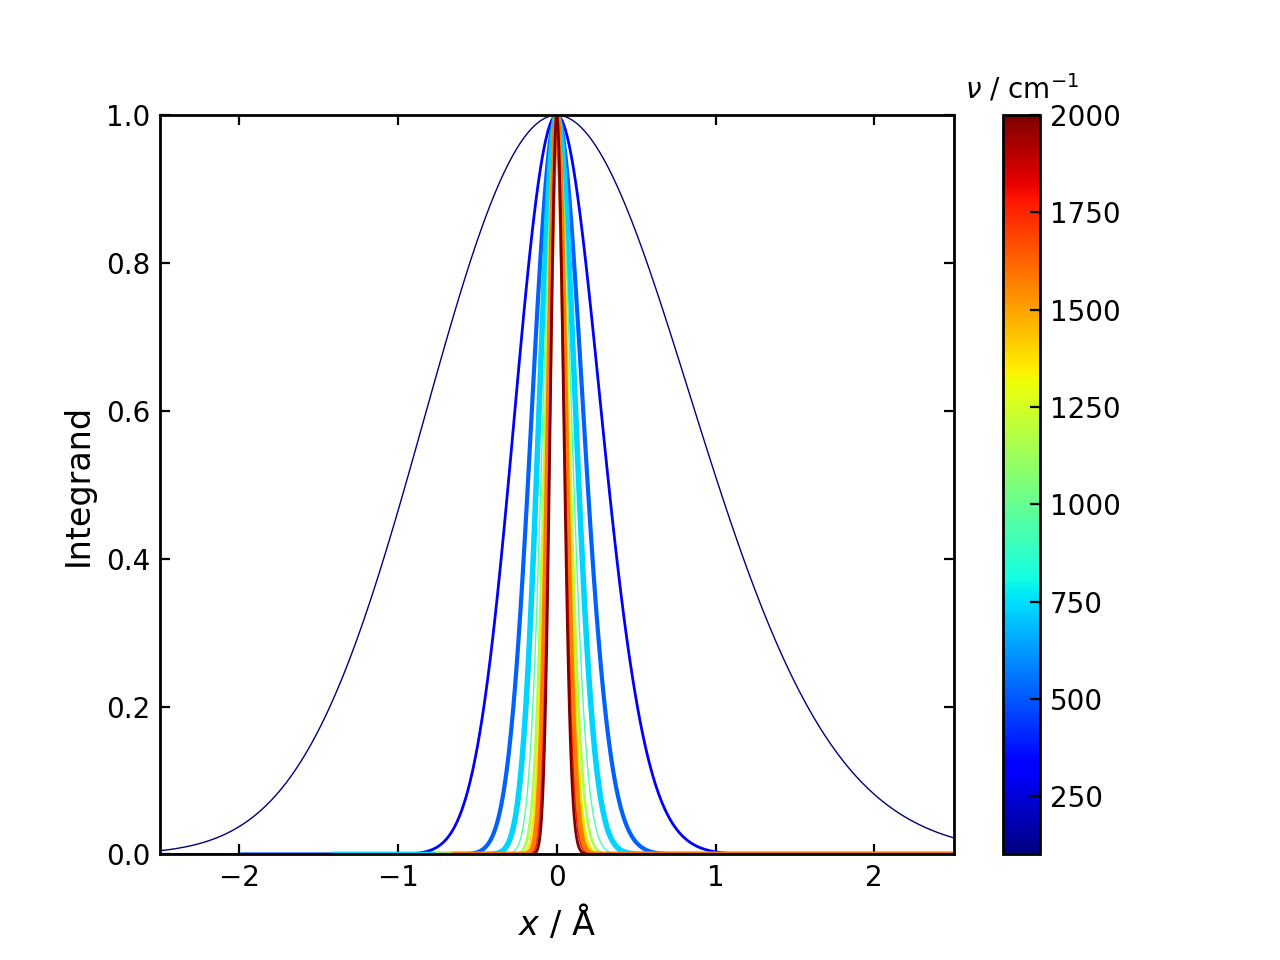
\includegraphics[width=12cm]{8/figs/morse_pf_integrand_vs_x}
	\vspace{0.2cm}
	\hrule
	\caption{Integrand of $Z_c$ vs $x$. $D_e$ = 400 kJ mol$^{-1}$, $T$ = 298.15 K, $m = 1$ amu.}
	\label{morse_pf_integrand_vs_x}
\end{figure}

\subsection{Exponential well}

To derive the entropy and internal energy due to translation of a molecule in an 3D exponential well the temperature derivative of the partition function ($Z_c^\text{exp}$) is required. For

\begin{equation}
	Z_c^\text{exp} =\left(\frac{2m\pi k_B T}{h^2} \right)^{3/2} \int_0^\infty 4\pi r^2 e^{- k(e^{ar} - 1) / k_B T} \; \text{d}r :=  \Lambda(T) I(T)
\end{equation}


\begin{equation}
	\begin{aligned}
		\left(\frac{\partial Z_c^\text{exp}}{\partial T}\right)_{N , V} &= \left(\frac{\partial \Lambda}{\partial T}\right)_{N , V} I(T) + \Lambda(T)\left(\frac{\partial I}{\partial T}\right)_{N , V} \\
		&= \Lambda(T) \frac{3}{2}T^{-1} I(T) + \Lambda(T) \int_0^\infty 4\pi r^2 \frac{k(e^{ar} - 1)}{k_B T^2}  e^{- k\beta (e^{ar} - 1)} \; \text{d}r \\
		&= \frac{3}{2T} Z_c^\text{exp} + \frac{\Lambda(T) k\beta}{T} \int_0^\infty 4\pi r^2 e^{ar}  e^{- k\beta(e^{ar} - 1)} \; \text{d}r \\
		&\qquad\qquad\qquad\qquad-  \frac{\Lambda(T) k\beta}{T}  \int_0^\infty 4\pi r^2 e^{- k\beta(e^{ar} - 1)} \; \text{d}r \\
		&= \frac{1}{T} \left(  \frac{3}{2} Z_c^\text{exp} + \Lambda(T) k\beta \int_0^\infty 4\pi r^2 e^{ar}  e^{- k\beta(e^{ar} - 1)} \; \text{d}r -  k\beta Z_c^\text{exp} \right) \\
		&= \frac{Z_c^\text{exp}}{T} \left( \frac{3}{2} - k\beta + \frac{\Lambda(T) k\beta}{Z_c^\text{exp}} \int_0^\infty 4\pi r^2 e^{ar}  e^{- k\beta(e^{ar} - 1)} \; \text{d}r
		\right)
	\end{aligned}
\end{equation}





\clearpage
\subsection{Test sets} \label{section::appendix_entropy_test_cases}

Test set {\bfseries{A}} contains two reactions from the Morita Baylis--Hillman reaction for which experimental reaction $\Delta S$ values are available (\tablename{ \ref{setA_data}}, \figurename{ \ref{plata_mbh}}).\cite{Plata2015}


\begin{table}[h!]
	\renewcommand{\arraystretch}{1.5}
	\begin{center}
		\small
		\begin{tabularx}{\textwidth}{YYYY} 
			\toprule
			Reaction & $T_\text{avg}$ / K & {$T\Delta S$} / \kcal & {$\Delta G$} / \kcal \\
			\hline
			% 4.184
			\bfseries{R-MBH1}       & 317.6  & -7.9 & -3.2\\
			\bfseries{R-MBH2}       & 328.4  & -10.2 & -3.9\\
			\bottomrule
		\end{tabularx}
	\end{center}
	
	\caption{Thermodynamic data for {\bfseries{A}}. No error is given. $T_\text{avg}$ values are averages over the temperature range used to calculate $\Delta S$.}
	\label{setA_data}
\end{table}

\begin{figure}[h!]
	\centering
	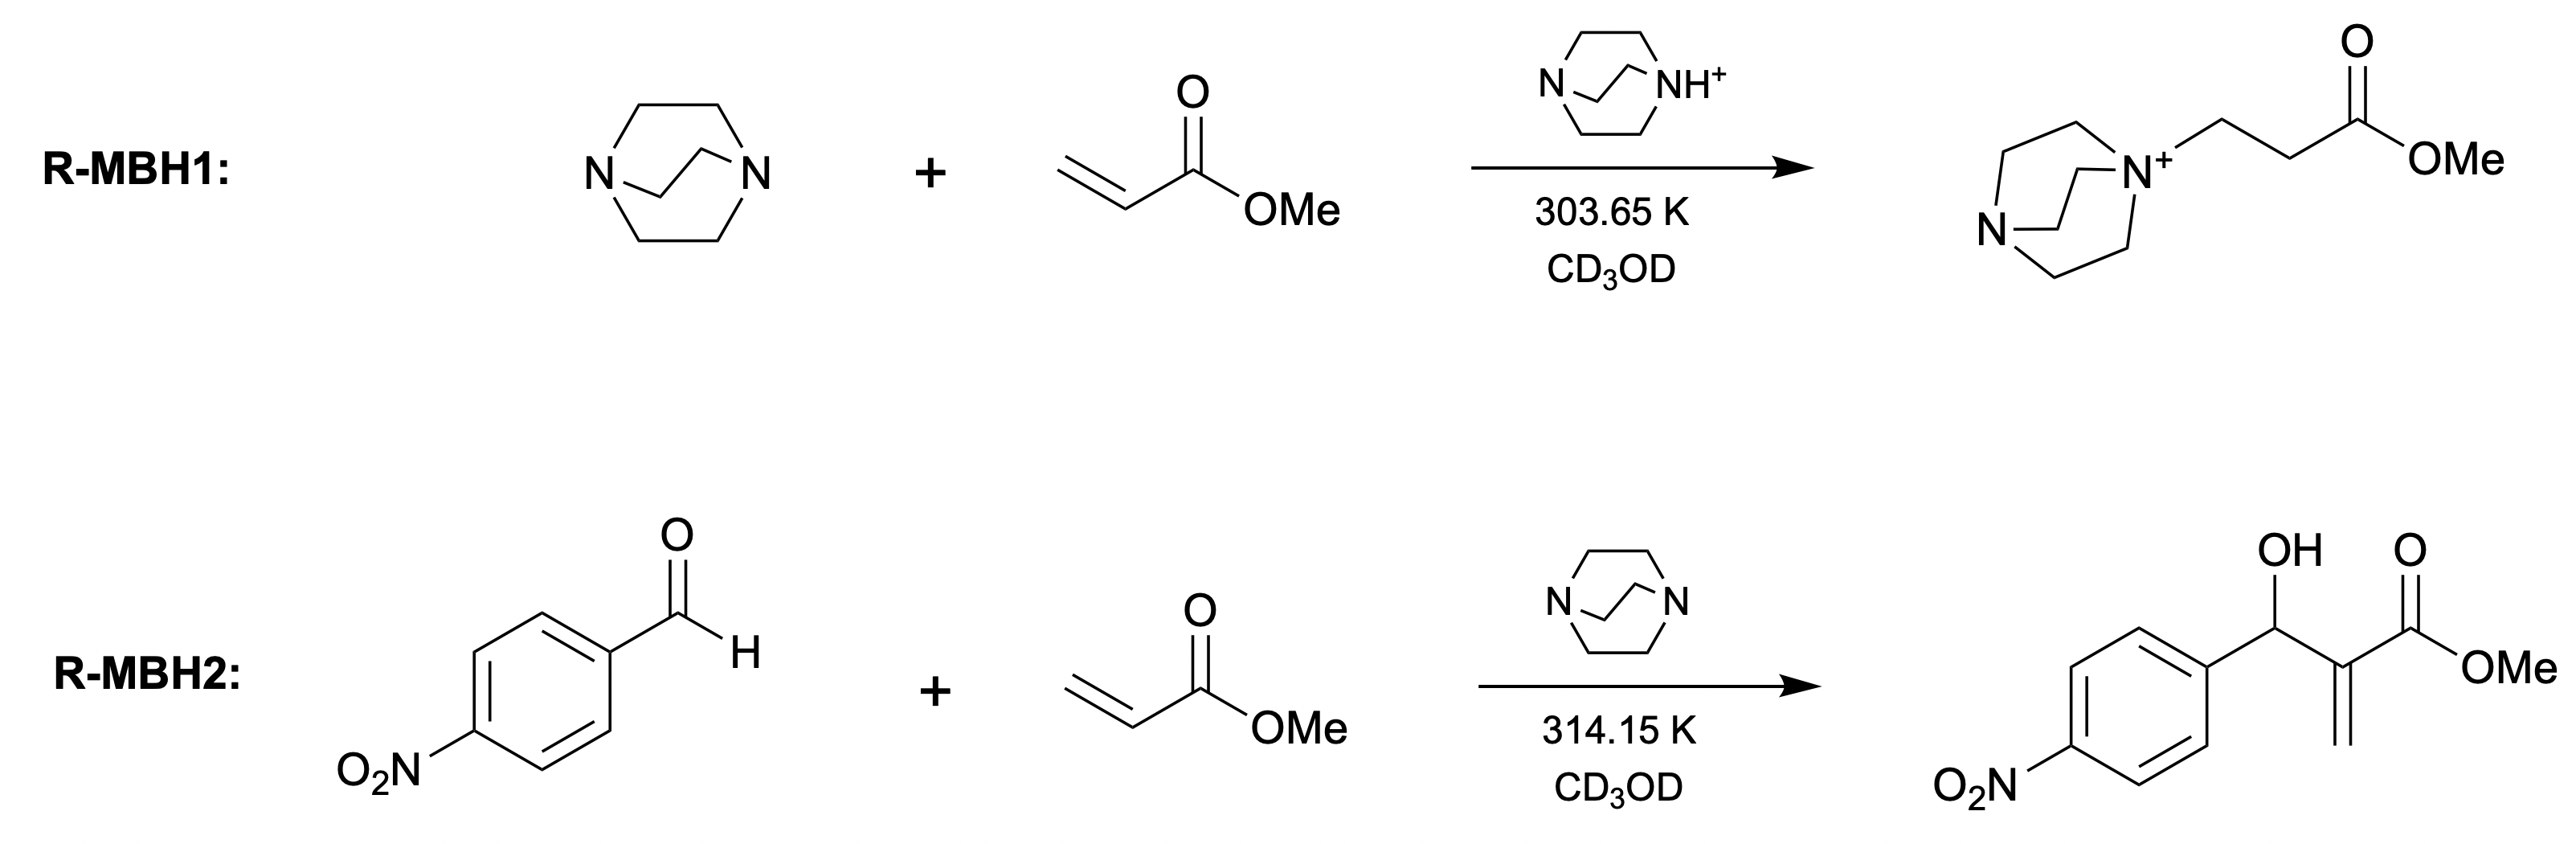
\includegraphics[width=13cm]{8/figs/plata_mbh}
	\vspace{0.2cm}
	\hrule
	\caption{Reactions in test set {\bfseries{A}}. }
	\label{plata_mbh}
\end{figure}

Test set {\bfseries{B}} comprise entropies of activation for 10 S$_\text{N}$2 reactions collated in ref. \cite{Vlasov2006} (\figurename{ \ref{vlasov_sn2}}).  These were chosen based on modest structural complexity, while spanning a wide range of $\Delta S^\ddagger$ values (\tablename{ \ref{setB_data}}).
\\
\begin{table}[h!]
	\renewcommand{\arraystretch}{1.5}
	\begin{center}
		\small
		\begin{tabularx}{\textwidth}{YYYYY} 
			\toprule
			Reaction & $T$ / K & {$\Delta H^\ddagger$} / \kcal & {$T\Delta S^\ddagger$} / \kcal & {$\Delta G^\ddagger$} / \kcal\\
			\hline
			\bfseries{R1} & 369.1 & 22.3 & -3.9 & 26.0\\
			\bfseries{R2} & 369.1 & 18.6 & -6.1 & 24.4\\
			\bfseries{R3} & 322.4 & 21.5 & -1.9 & 23.4\\
			\bfseries{R4} & 303.1 & 15.9 & -3.7 & 19.6\\
			\bfseries{R5} & 303.1 & 16.5 & -2.1 & 18.6\\
			\bfseries{R6} & 303.1 & 16.4 & -4.9 & 21.3\\
			\bfseries{R7} & 303.1 & 18.5 & -2.0 & 20.5\\
			\bfseries{R8} & 252.2 & 11.9 & -3.1 & 15.0\\
			\bfseries{R9} & 303.1 & 18.6 & -2.4 & 20.9\\
			\bfseries{R10} & 303.1 & 20.2 & -1.3 & 21.5\\
			\bottomrule
		\end{tabularx}
	\end{center}
	
	\caption{Activation parameters for test set {\bfseries{B}}. Reactions are shown in \figurename{ \ref{vlasov_sn2}}. Where errors are quoted: ${\Delta S}_\text{err} < \pm2.5$ J K$^{-1}$ mol$^{-1}$, ${\Delta H}_\text{err} < \pm0.2$ \kcal.}
	\label{setB_data}
\end{table}

\begin{figure}[h!]
	\centering
	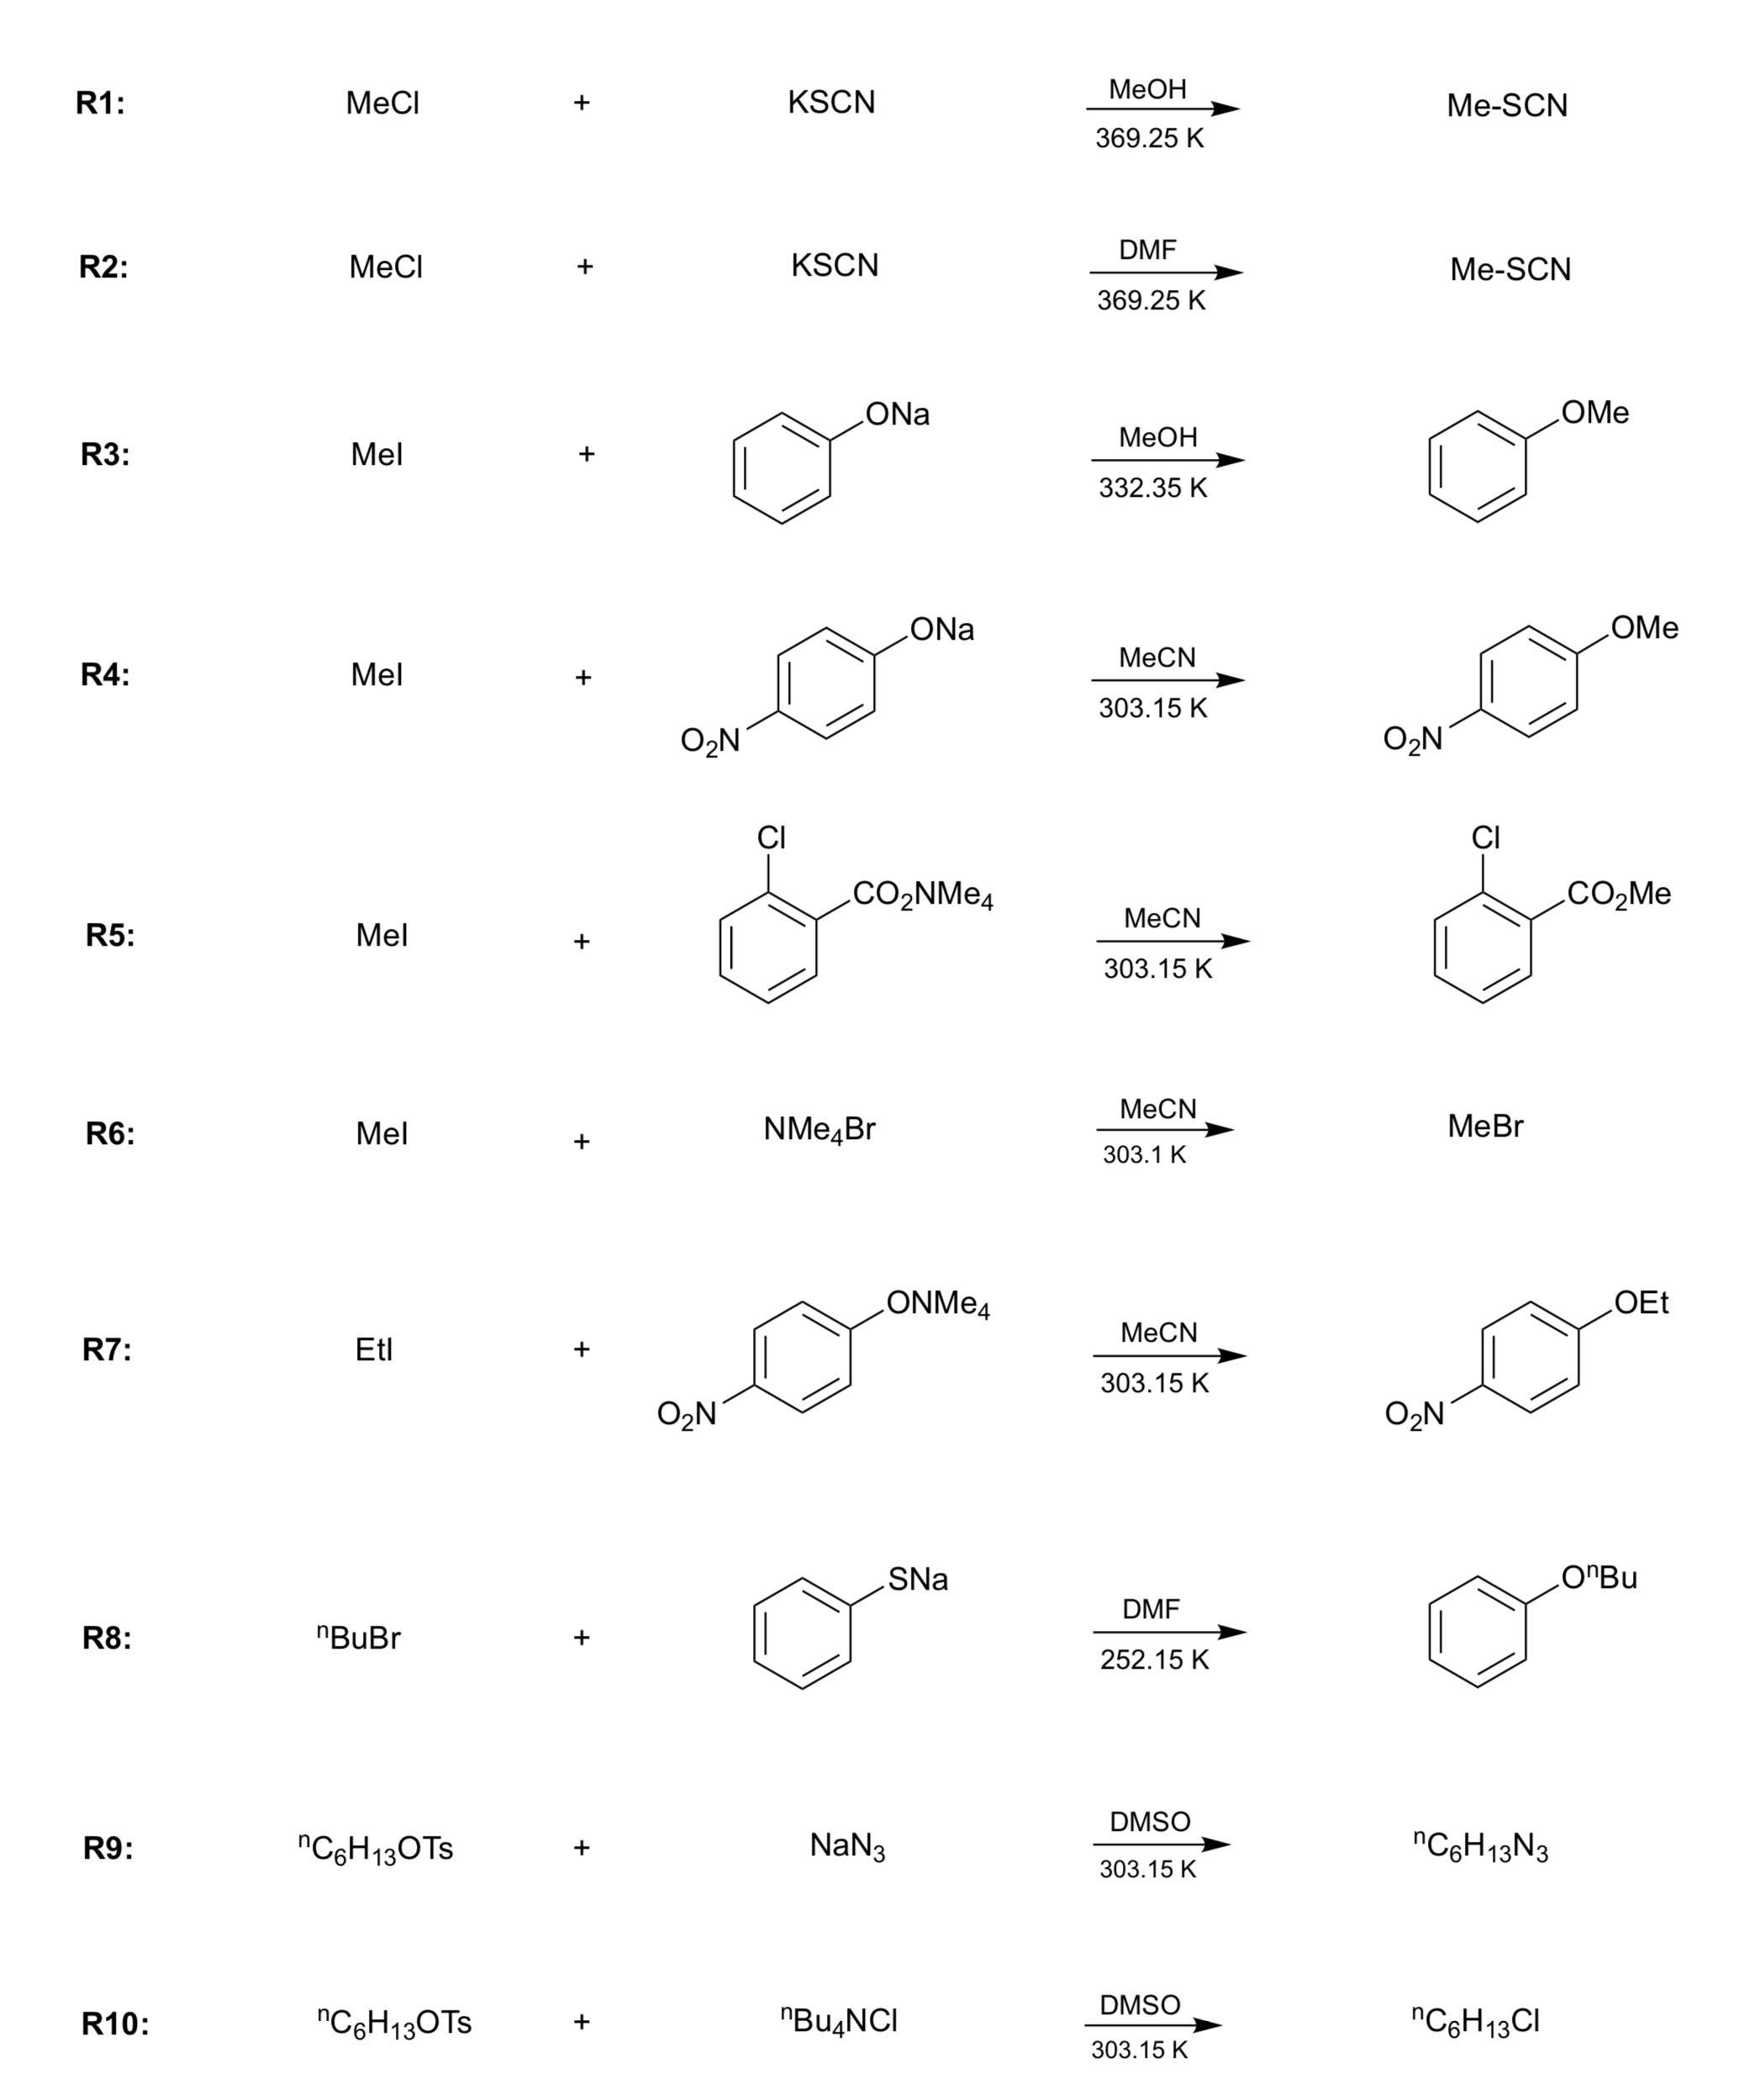
\includegraphics[width=14.5cm]{8/figs/vlasov_sn2}
	\vspace{0.2cm}
	\hrule
	\caption{Reactions in test set {\bfseries{B}}.}
	\label{vlasov_sn2}
\end{figure}


\clearpage
\end{document}